\documentclass[11pt]{article}
\usepackage{fullpage}
\usepackage{amsfonts}
\usepackage{amssymb}
\usepackage{mdwlist}
\usepackage[usenames,dvipsnames]{xcolor}
\usepackage{tikz}
\usepackage{enumerate}


\newcommand{\coursenum}{CS172}
\newcommand{\coursename}{Automata, Computability and Complexity}
\newcommand{\courseprof}{Professor Luca Trevisan}

%       Usage: \ptitle{title}{dateout}
\newcommand{\ptitle}[2]{\noindent\parbox{\textwidth}
{U.C. Berkeley --- \coursenum : \coursename \hfill #1 \newline
\courseprof \hfill #2 \newline
\mbox{}\hrulefill\mbox{}}\vspace*{1ex}\mbox{}\newline
\bigskip
\begin{center}{\Large\bf #1}\end{center}
\bigskip}


%       Usage: \handout{title}{datelec}{dateout}{scribe}
\newcommand{\handout}[2]{\thispagestyle{empty}
 \markboth{Notes for Lecture #1}{Notes for Lecture #1}
 \pagestyle{myheadings}\htitle{#1}{#2}}

%       Usage: \pset{title}{dateout}
\newcommand{\pset}[2]{\thispagestyle{empty}
 \markboth{#1 --- #2}{#1 --- #2}
 \pagestyle{myheadings}\ptitle{#1}{#2}}



\begin{document}
\ptitle{Problem Set 3}{February 5, 2015}
This problem set is due on Friday, February 13, by 5pm. Please submit your solution online using bcourses,
as a pdf file.
You can type your solution, or handwrite it. If you handwrite it, then either
scan it or take a good resolution picture of each page and then collate the pictures
and export them to a {\em single} pdf file.
\bigskip
\hrule



\section*{Problem 1: Minimal Automata (10/100)}
Consider the language $L=\{x\in\{0,1\}^*:$ the number of 1's in $x$ is a multiple of 3$\}$.  Draw a minimal DFA with states labeled with the equivalence classes [$\varepsilon$], [1], and [11] defined by indistinguishability over $L$.

\section*{Problem 2: Regular? (20/100)}

Are the following languages regular?  If so, draw a minimal DFA for it with each state labeled with its corresponding equivalence class (signified by a representative for that class under the indistinguishability relation).  If not, prove this with the Myhill-Nerode theorem by exhibiting infinitely many distinguishable strings.

\begin{enumerate}[a)]
\item $L=\{x\in\{a,b\}^*:$ the number of $b$'s in $x$ has a remainder of 3 when divided by 5$\}$

\item $L=\{x\in\{a,b\}^*:$ the number of $a$'s in $x$ is twice the number of $b$'s in $x\}$

\item $L=\{x\oplus y\ominus z:x,y,z\in\{0,1\}^*,$ bin$(x)+$bin$(y)=$bin$(z)\}$ for $\Sigma=\{0,1,\oplus,\ominus\}$.  And bin$(x)$ for $x\in\{0,1\}^*$ is the number associated with $x$ when interpreted as a binary number.

\item $L=\{x\in\{0,1\}^*: x$ ends in 101$\}$
\end{enumerate}



\section*{Problem 3: State Minimization (30/100)}

Consider the following automaton.  Find the minimal equivalent DFA.\\

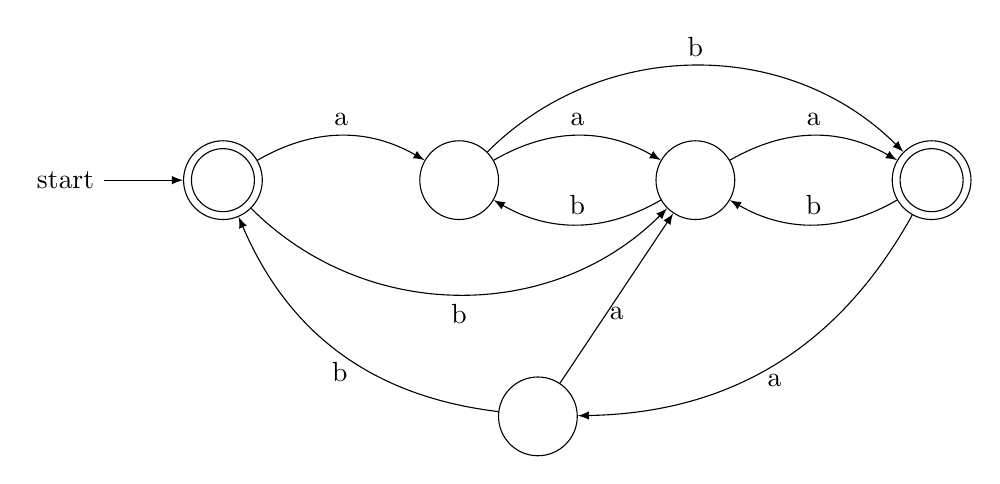
\begin{tikzpicture}

\node[draw,circle,minimum size=1cm] (node0) at (0,0) {};
\node[draw,circle,minimum size=.8cm] at (0,0) {};

\node[draw,circle,minimum size=1cm] (node1) at (3,0) {};

\node[draw,circle,minimum size=1cm] (node2) at (6,0) {};

\node[draw,circle,minimum size=1cm] (redundant0) at (9,0) {};
\node[draw,circle,minimum size=.8cm] at (9,0) {};

\node[draw,circle,minimum size=1cm] (redundant1) at (4,-3) {};


\node (label) at (-2, 0) {start};
\path [-latex] (label) edge (node0);

\path [-latex] (node0) edge [bend left] node[above] {a} (node1);
\path [-latex] (node0) edge [bend right=45] node[below] {b} (node2);

\path [-latex] (node1) edge [bend left=45] node[above] {b} (redundant0);
\path [-latex] (node1) edge [bend left] node[above] {a} (node2);

\path [-latex] (node2) edge [bend left] node[above] {b} (node1);
\path [-latex] (node2) edge [bend left] node[above] {a} (redundant0);

\path [-latex] (redundant0) edge [bend left] node[below] {a} (redundant1);
\path [-latex] (redundant0) edge [bend left] node[above] {b} (node2);

\path [-latex] (redundant1) edge [bend left] node[below] {b} (node0);
\path [-latex] (redundant1) edge node[below] {a} (node2);
\end{tikzpicture}


\section*{Problem 4: Classes (40/100)}

Let $k$ be an integer, and define $L_k$ to be the language of strings
over $\{ 0,1\}$ that have a 1 in the $k$th-to-last position. Prove that $L_k$ is regular and that every DFA for $L_k$ has exponentially many states with respect to $k$.  Prove that $L_k$ has an NFA with $O(k)$ states and a Regular Expression of length $O(k)$.

\end{document}